\documentclass[border=5pt]{standalone}
\usepackage{fontspec}
\usepackage{unicode-math}
\setmainfont{Noto Serif}
\newfontfamily\FigureItalic{Noto Serif}
\setmathfont{STIXTwoMath-Regular.otf}
\usepackage{tikz}
\usetikzlibrary{arrows.meta,calc,patterns,decorations.pathmorphing,decorations.markings,decorations.pathreplacing,positioning,backgrounds}
\definecolor{Ink}{HTML}{000000}
\definecolor{Curve}{HTML}{000000}
\definecolor{Bzero}{HTML}{000000}
\definecolor{Bone}{HTML}{000000}
\definecolor{Btwo}{HTML}{000000}
\definecolor{Bthree}{HTML}{000000}
\definecolor{Bfour}{HTML}{000000}
\tikzset{
 ax/.style={draw=Ink,line width=.72pt,-{Latex[length=2.4mm,width=1.5mm]}},
 lev/.style={draw=Ink,line width=1.4pt,line cap=butt},
 thinlev/.style={draw=Ink,line width=.65pt,line cap=butt},
 helper/.style={draw=Ink,line width=.65pt},
 bare/.style={draw=Ink,line width=.95pt,dash pattern=on 4pt off 2.8pt},
 curve/.style={draw=Ink,line width=1.85pt,line cap=round,line join=round},
 ray/.style={draw=Ink,line width=1.0pt,-{Latex[length=2.3mm,width=1.4mm]}},
 measure/.style={draw=Ink,line width=.75pt,{Latex[length=1.9mm,width=1.2mm]}-{Latex[length=1.9mm,width=1.2mm]}},
 link/.style={draw=Ink,line width=1.0pt},
 wave/.style={draw=Ink,line width=.85pt,decorate,decoration={snake,amplitude=.33mm,segment length=2.5mm,pre length=.8mm,post length=.8mm}},
 photon/.style={draw=Ink,line width=1.0pt,-{Latex[length=2.0mm,width=1.3mm]},decorate,decoration={snake,amplitude=.4mm,segment length=2.7mm,pre length=0mm,post length=1.9mm}},
 lab/.style={text=Ink,font=\fontsize{13.5}{16}\selectfont,inner sep=2pt},
 small/.style={text=Ink,font=\fontsize{11.5}{14}\selectfont,inner sep=2pt},
 tag/.style={text=Ink,font=\fontsize{14}{17}\selectfont\FigureItalic\itshape,inner sep=2pt}}
\pagestyle{empty}

\begin{document}
% Figure 13.9; source-grounded revision.
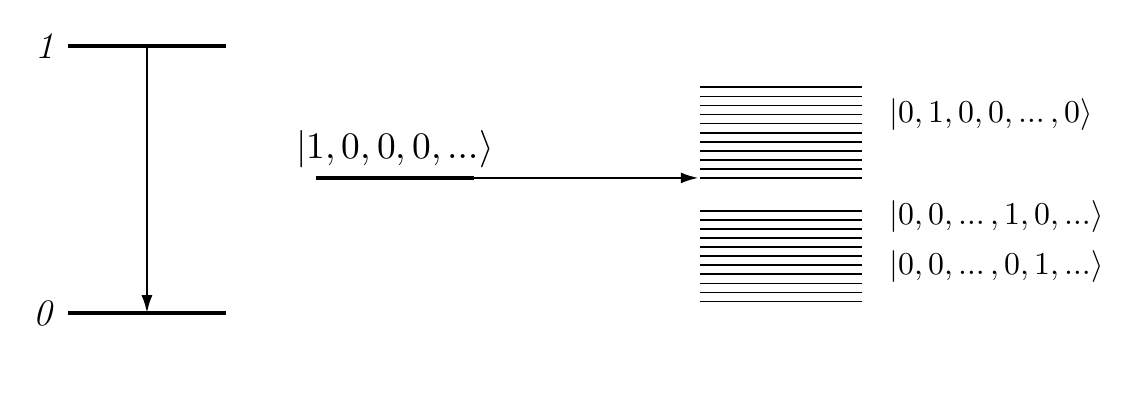
\begin{tikzpicture}[x=1cm,y=1cm]
\coordinate (a0) at (1.15000,0.00000);
\coordinate (a0L) at (0.15000,0.00000);
\coordinate (a0R) at (2.15000,0.00000);
\draw[lev] (a0L) -- (a0R);
\node[lab,anchor=east] at (0.05000,0.00000) {\textit{0}};
\coordinate (a1) at (1.15000,3.40000);
\coordinate (a1L) at (0.15000,3.40000);
\coordinate (a1R) at (2.15000,3.40000);
\draw[lev] (a1L) -- (a1R);
\node[lab,anchor=east] at (0.05000,3.40000) {\textit{1}};
\draw[ray] (a1) -- (a0);
\node[tag] at (1.15000,-0.65000) {а};
\coordinate (exc) at (4.30000,1.72000);
\coordinate (excL) at (3.30000,1.72000);
\coordinate (excR) at (5.30000,1.72000);
\draw[lev] (excL) -- (excR);
\node[lab] at (4.30000,2.08000) {$|1,0,0,0,\ldots\rangle$};
% Two continuum sectors, rather than a uniform uninterrupted ladder.
% These are schematic bands: ticks are NOT distinct measured frequencies.
\foreach \j in {0,...,10}{
  \pgfmathsetmacro{\ylow}{.15+.115*\j}
  \draw[thinlev] (8.175,\ylow)--(10.225,\ylow);
}
\foreach \j in {0,...,10}{
  \pgfmathsetmacro{\yhigh}{1.72+.115*\j}
  \draw[thinlev] (8.175,\yhigh)--(10.225,\yhigh);
}
% One atomic transition excites the compound continuum; it terminates on
% the appropriate band and never in the blank gap between bands.
\draw[ray] (excR) -- (8.16,1.72);
\node[small,anchor=west] at (10.50,2.52) {$|0,1,0,0,\ldots,0\rangle$};
\node[small,anchor=west] at (10.50,1.23) {$|0,0,\ldots,1,0,\ldots\rangle$};
\node[small,anchor=west] at (10.50,.60) {$|0,0,\ldots,0,1,\ldots\rangle$};
\node[tag] at (9.20000,-0.65000) {б};\end{tikzpicture}

\end{document}
